Se presentarán las matrices morfológicas de cada uno de los dominios y cómo se conectan para dar formas a los 3 conceptos de solución.
%%% FIGURA LEYENDA
\begin{figure}[H]
        \centering       
        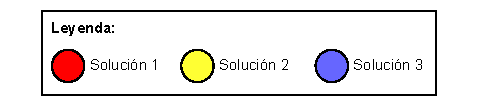
\includegraphics[width=0.4\textwidth]{ANNEX/Fig/AE_0-Leyenda.pdf}
        \label{fig:Annex_E_Leyenda}
\end{figure}
%%% FIGURA 1/7
\begin{figure}[H]
        \centering       
        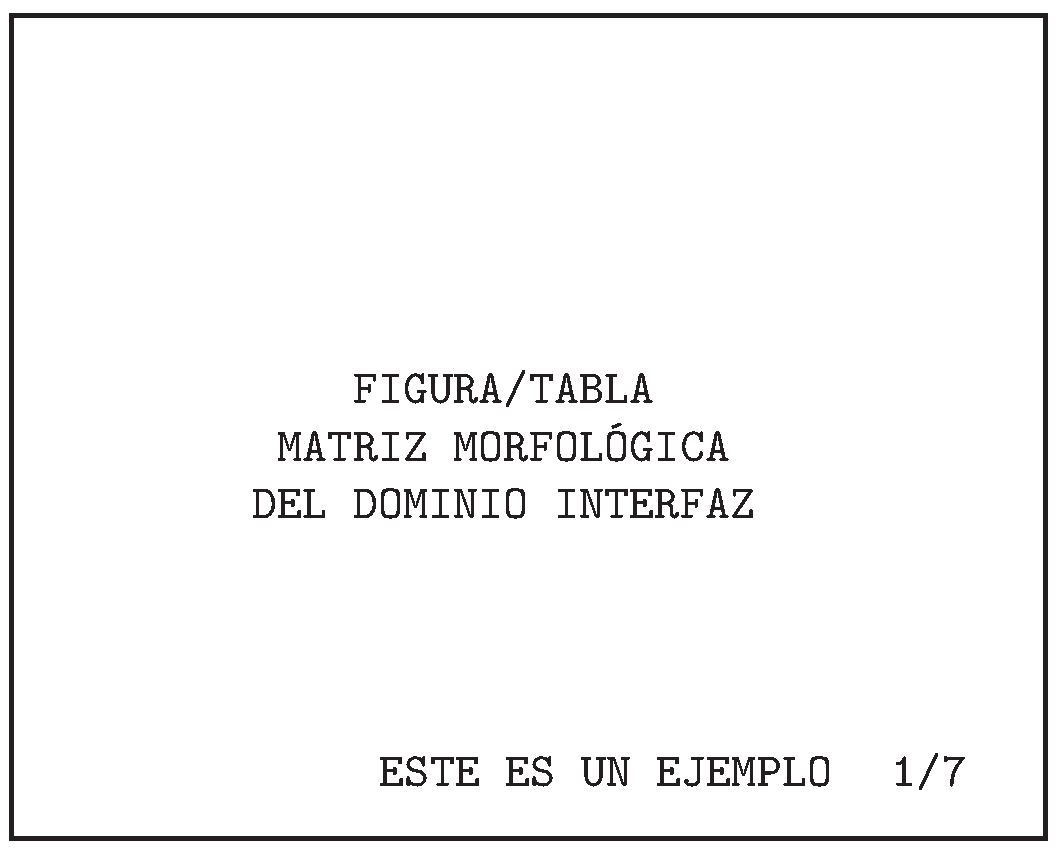
\includegraphics[width=0.7\textwidth]{ANNEX/Fig/AE_MatrizMorfologica-01-Dominio-Interfaz.pdf}
        \caption{Matriz morfológica para la interfaz del sistema}
        \label{fig:Annex_E_MatrizMorfologica-01-Interfaz}
\end{figure}
%%% FIGURA 2/7
\begin{figure}[H]
        \centering       
        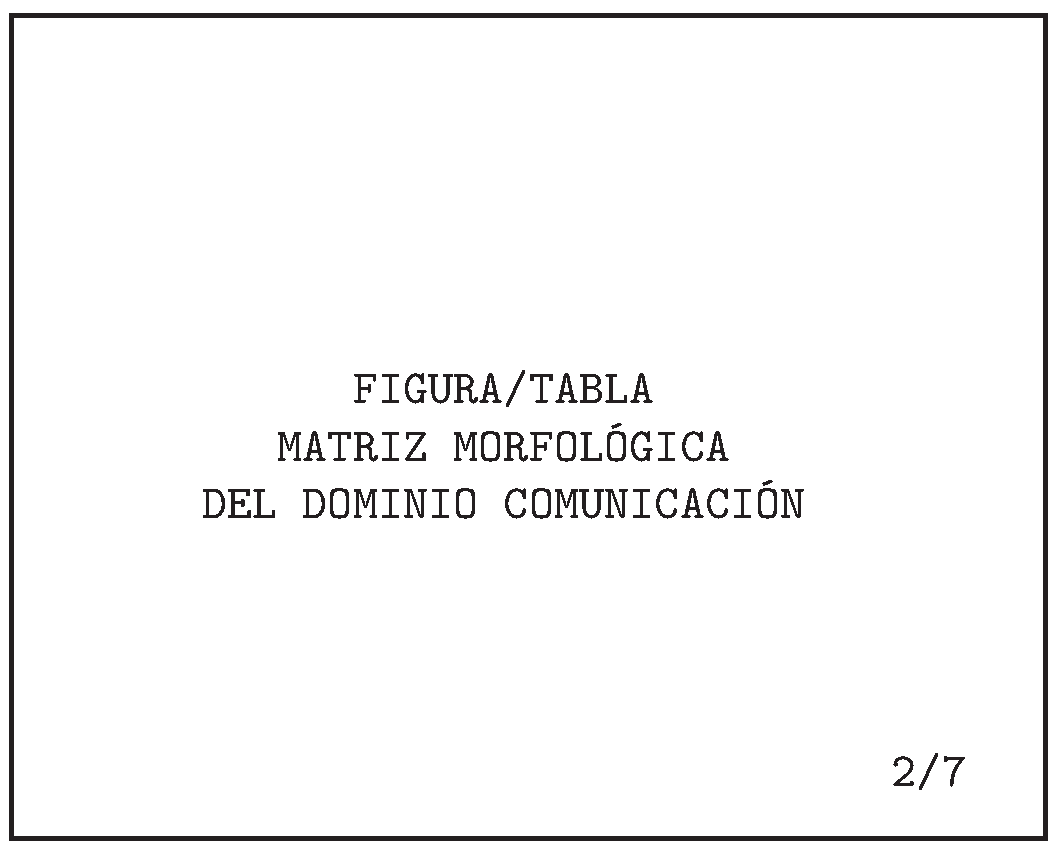
\includegraphics[width=0.7\textwidth]{ANNEX/Fig/AE_MatrizMorfologica-02-Dominio-Comunicacion.pdf}
        \caption{Matriz morfológica del dominio de comunicación}
        \label{fig:Annex_E_MatrizMorfologica-02-Comunicacion}
\end{figure}
%%% FIGURA 3/7
\begin{figure}[H]
        \centering       
        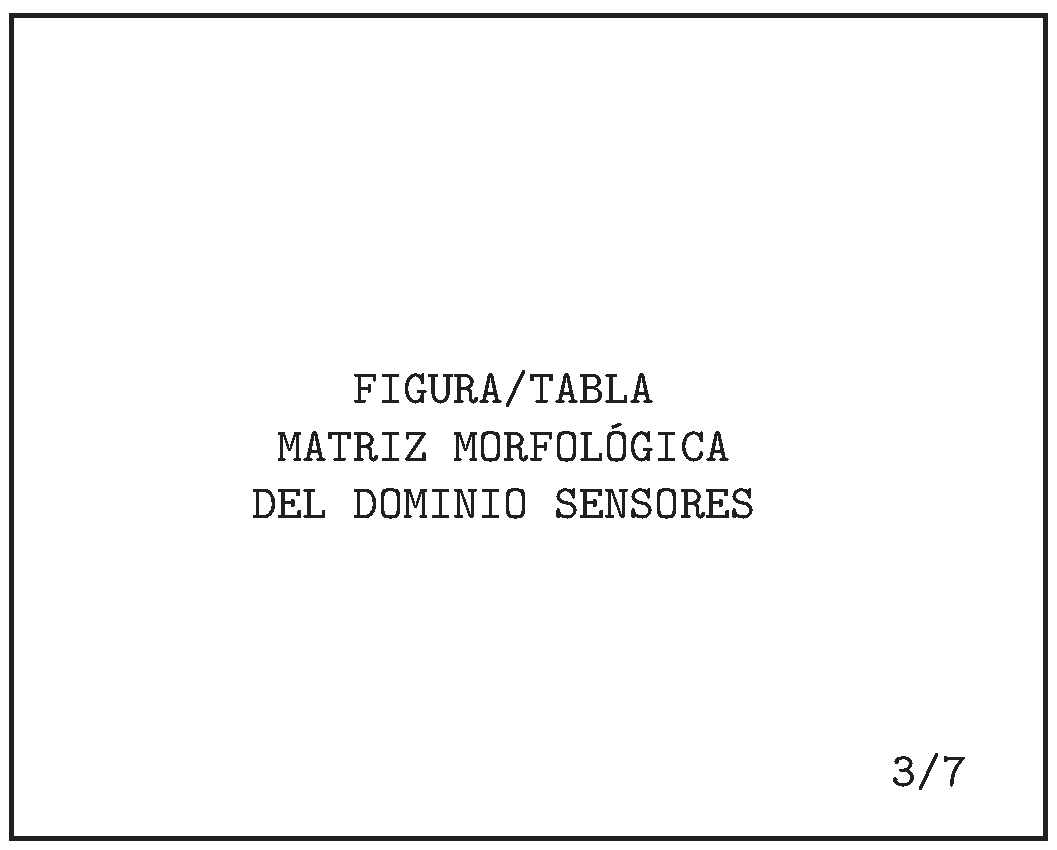
\includegraphics[width=0.7\textwidth]{ANNEX/Fig/AE_MatrizMorfologica-03-Dominio-Sensores.pdf}
        \caption{Matriz morfológica del dominio de sensores}
        \label{fig:Annex_E_MatrizMorfologica-03-Sensores}
\end{figure}
%%% FIGURA 4/7
\begin{figure}[H]
        \centering       
        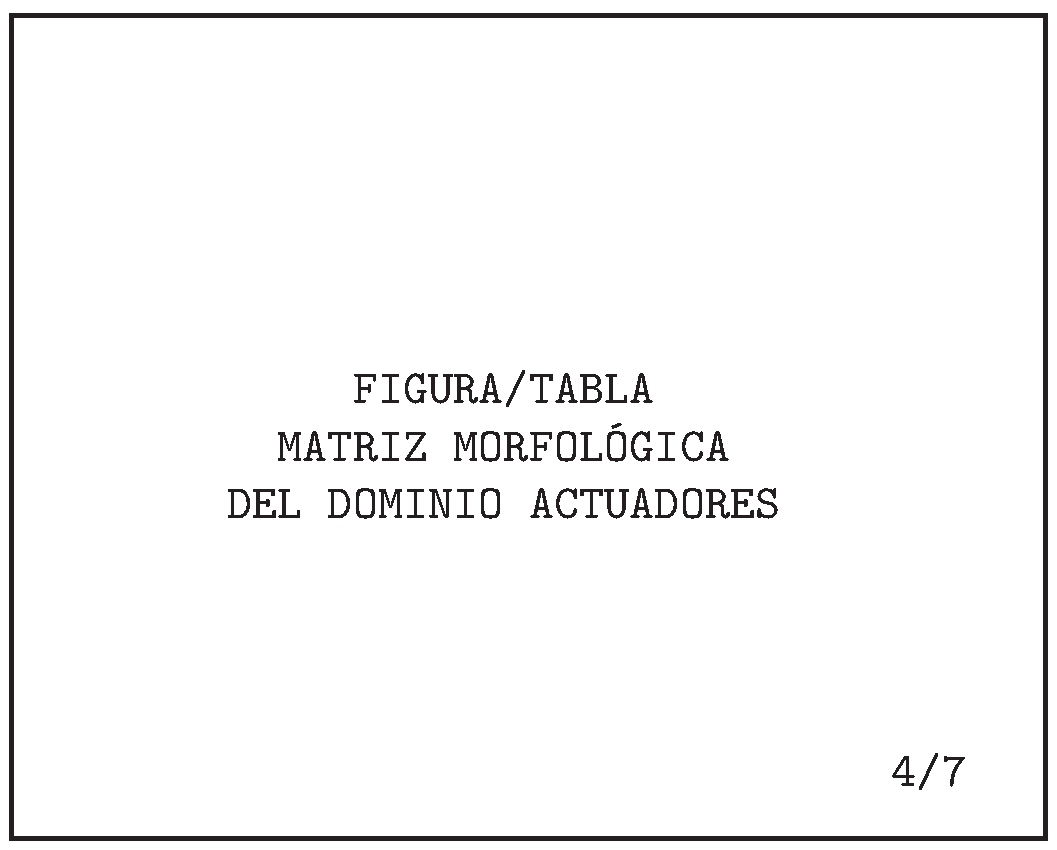
\includegraphics[width=0.7\textwidth]{ANNEX/Fig/AE_MatrizMorfologica-04-Dominio-Actuadores.pdf}
        \caption{Matriz morfológica del dominio de actuadores}
        \label{fig:Annex_E_MatrizMorfologica-04-Actuadores}
\end{figure}
%%% FIGURA 5/7
\begin{figure}[H]
        \centering       
        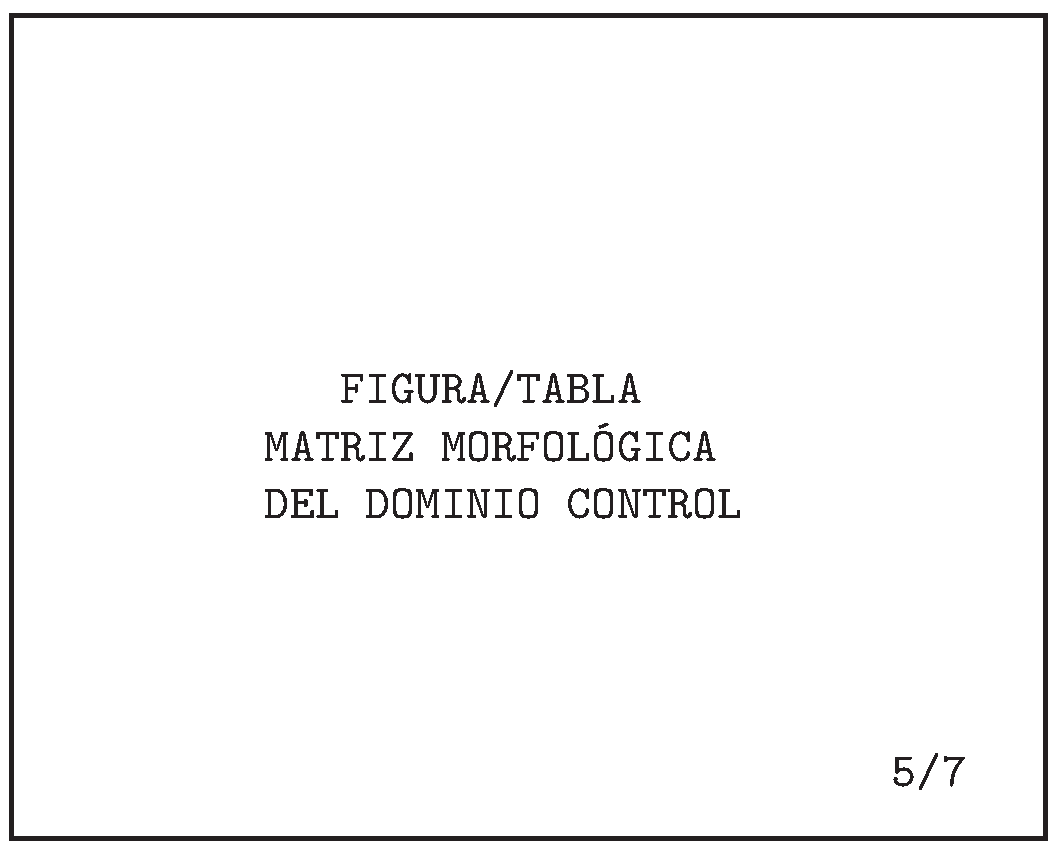
\includegraphics[width=0.7\textwidth]{ANNEX/Fig/AE_MatrizMorfologica-05-Dominio-Control.pdf}
        \caption{Matriz morfológica del dominio de control}
        \label{fig:Annex_E_MatrizMorfologica-05-control}
\end{figure}
%%% FIGURA 6/7
\begin{figure}[H]
        \centering       
        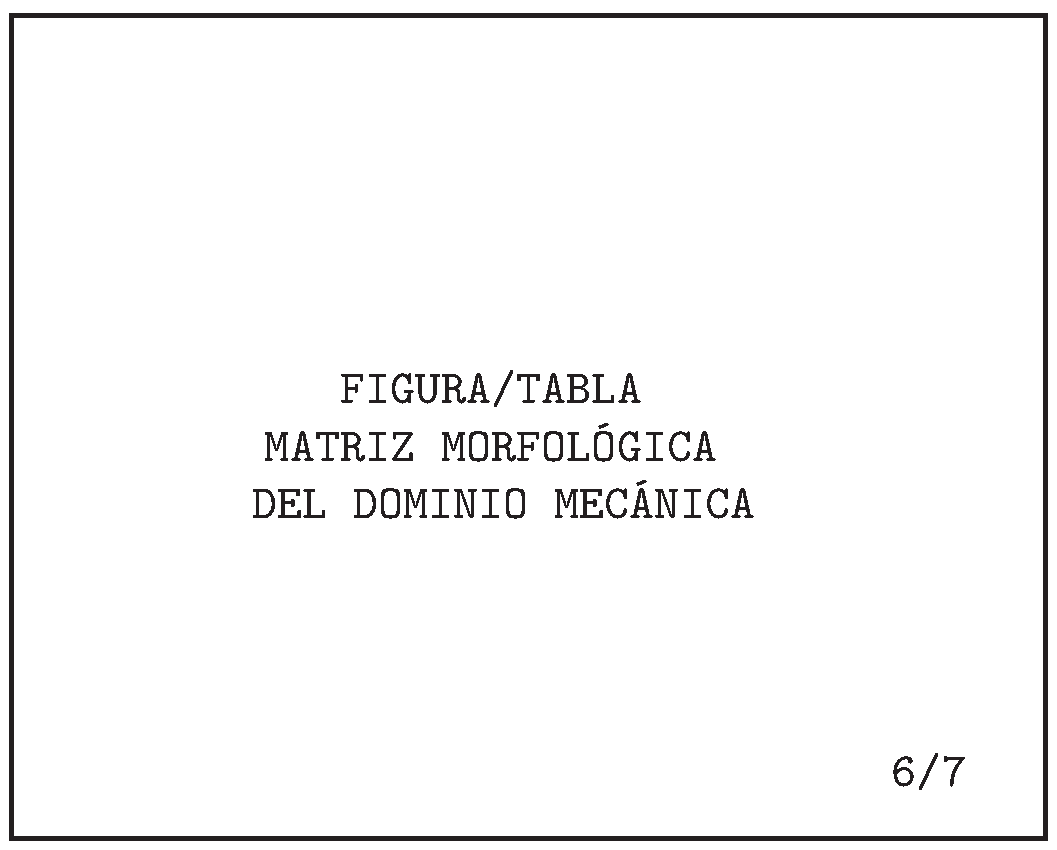
\includegraphics[width=0.7\textwidth]{ANNEX/Fig/AE_MatrizMorfologica-06-Dominio-Mecanica.pdf}
        \caption{Matriz morfológica del dominio de mecánica}
        \label{fig:Annex_E_MatrizMorfologica-06-Mecanica}
\end{figure}
%%% FIGURA 7/7
\begin{figure}[H]
        \centering       
        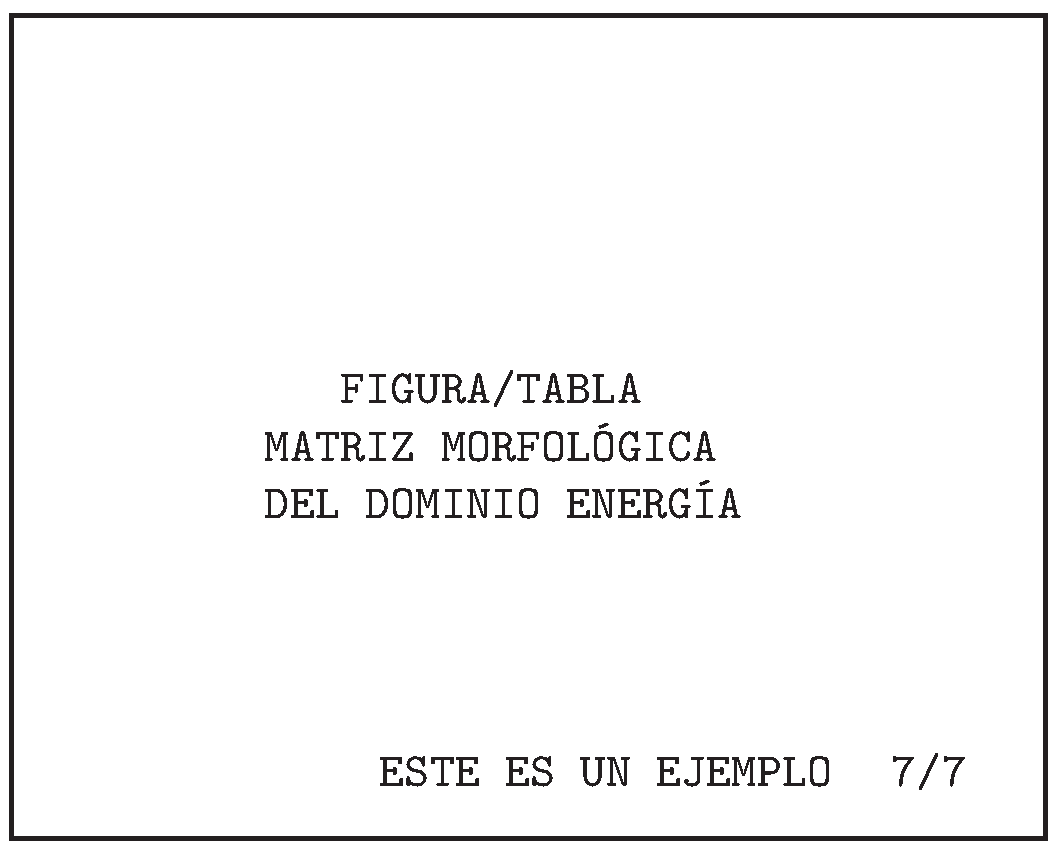
\includegraphics[width=0.7\textwidth]{ANNEX/Fig/AE_MatrizMorfologica-07-Dominio-Energia.pdf}
        \caption{Matriz morfológica del dominio de energía}
        \label{fig:Annex_E_MatrizMorfologica-07-Energia}
\end{figure}
